%!TEX root = /Users/louis/Documents/PhD/Deliverables/Thesis/thesis.tex

\section{MDE Guidelines and Methods}
\label{sec:mde_methods}
For performing MDE, new engineering practices and processes have been proposed. Proponents of MDE have produced guidance and methods for MDE. This section discusses the guidance for MDE set out in the Model-Driven Architecture \cite{mda} and the methods for MDE described in \cite{stahl06mdsd,kelly08dsm,greenfield04software}. 

\subsection{The Model-Driven Architecture}
The Model-Driven Architecture (MDA) is a software engineering framework defined by the OMG. The MDA provides guidelines for MDE. For instance, the MDA prescribes the use of a Platform Independent Model (PIM) and one or more Platform Specific Models (PSMs).

A PIM provides an abstract, implementation-agnostic view of a system. Successive PSMs provide increasingly more implementation detail. Inter-model mappings are used to forward- and reverse-engineer these models, as depicted in
Figure \ref{fig:mda}.

\begin{figure}[htbp]
  \begin{center}
    \leavevmode
    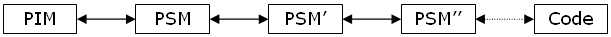
\includegraphics[scale=0.5]{2.Background/images/PIMs_and_PSMs.png}
  \end{center}
  \caption{Interactions between a PIM and several PSMs.}
  \label{fig:mda}
\end{figure}

A key difference between the MDA and related approaches, such as round-trip engineering (in which models and code are co-evolved to develop a system), is that the MDA prescribes automated transformations between PIM and PSMs, whereas other approaches use some manual transformations.

With MDA, the OMG sought to communicate and encourage the adoption of MDE principles, and to provide standards for building interoperable MDE platforms. Arguably, some parts of MDA have been widely adopted. For example, the metamodelling language provided by EMF is heavily based on MOF (Section~\ref{subsec:mof}), one of the key standards prescribed by MDA. However, it is difficult to assess the extent to which the principles advocated by MDA have been adopted. Empirical analysis is needed to determine the way in which MDE is performed in practice, and to drive changes to MDA and the modelling standards provided by the OMG.

\subsubsection{Standards for the MDA}
As part of the guidelines for MDE, the OMG prescribes a set of standards for the MDA. The standards are allocated to one of four tiers, and each tier represents a different level of model abstraction (Figure \ref{fig:mda-pyramid}). Members of one tier conform to a member of the tier above. A discussion of the four tiers, based on \cite[Section 8.2]{kleppe03mda}, follows.

\begin{figure}[htbp]
  \begin{center}
    \leavevmode
    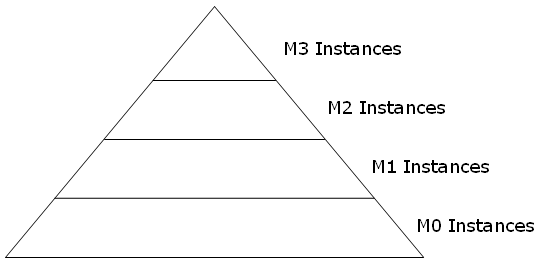
\includegraphics[scale=0.5]{2.Background/images/mda-pyramid.png}
  \end{center}
  \caption{The tiers of standards used as part of MDA.}
  \label{fig:mda-pyramid}
\end{figure}

The base of the pyramid, tier M0, contains the domain (real-world). When modelling a business, this tier is used to describe items of the business itself, such as a real customer or an invoice. When modelling software, M0 instances describe the software representation of such items. M1 contains models (Section~\ref{subsec:models}) of the concepts in M0, for example a customer may be represented as a class with attributes. The M2 tier contains the modelling languages (metamodels, Section~\ref{subsec:modelling_languages}) used to describe the contents of the M1 tier. For example, if UML \cite{uml212} models were used to describe concepts as classes in the M1 tier, M2 would contain the UML metamodel. Finally, M3 contains a metamodelling language (metametamodel, Section~\ref{subsec:mof}) which describes the modelling languages in the M2 tier. As discussed in Section~\ref{subsec:mof}, the M3 tier facilitates tool standardisation and interoperability. The MDA specifies the Meta-Object Facility (MOF) \cite{mof} as the only member of the M3 tier.

\subsubsection{Interpretations of the MDA}
\cite{mcneile03mda} identifies two ways in which engineers have interpreted the MDA. Both interpretations begin with a PIM, but the way in which executable code is produced differs:

\begin{itemize}
 \item \textbf{Translationist}: The PIM is used to generate code directly using a sophisticated code generator. Any intermediate PSMs are internal to the code generator. No generated artefacts are edited manually.
 \item \textbf{Elaborationist}: Any generated artefacts (such as PSMs, code and documentation) can be augmented with further details of the application. To ensure that all models and code are synchronised, tools must allow bi-directional transformations.
\end{itemize}

Translationists must encode behaviour in PIMs \cite{mellor02executable}, whereas elaborationists have a choice, electing to specify behaviour in PSMs or in code \cite{kleppe03mda}.

The difference between translationist and elaborationist approaches to MDE is related to a difference in the way in which models are viewed in traditional approaches to software engineering. For example, \cite{evans04domain} proposes the use of models throughout the development process, and the way in which code is structured is driven by the model. By contrast, \cite[ch. 14]{martin06agile} prescribes modelling only for communicating and reasoning about a design, and not ``as a long-term replacement for real, working software''. Rather \cite{martin06agile} advocate using models to quickly compare different ways in which a system might be structured and then disregarding those models in favour of working code.

\subsubsection{Use of MDA}
The guidelines set out in the MDA have been adopted -- in varying degrees -- by the methods for MDE described in the sequel. Tools for MDE (Section~\ref{sec:mde_tools}) tend not to enforce many of the MDA guidelines. For example, contemporary modelling frameworks allow -- but do not force -- developers to specify a single PIM and use model transformation to create successive PSMs. The MDE standards prescribed by the MDA have been widely adopted. MOF, UML and XMI, for example, are used in many contemporary modelling frameworks and modelling tools. 

% \subsection{Models in Software Engineering}
% 
% \emph{\textbf{Richard, Fiona}: This section is the result of reconciling an argument  I was having with myself! I agree with most of the principles in \cite{martin06agile}, but disagree that code should always be preferred to models. It took me quite a while to come to the conclusions reached in this section, but I'm not sure if the section adds enough value to warrant inclusion in the thesis.} \vspace{4mm}
% 
% The models that \cite{jackson95software} describes are used widely in software engineering. This section considers two software engineering approaches, each with  different opinions of the role of models in software engineering. \cite{evans04domain} advocates modelling throughout software development to better understand the object system, and prescribes structuring software based on the terms and concepts identified in the object system. \cite{martin06agile} advocates that the primary product of software engineering is code, and as such, models should be used to explore ideas, but then disregarded in favour of code.
% 
% \subsubsection{In Favour of Modelling}
% \cite{evans04domain} proposes the use of models throughout the development process to capture and communicate knowledge of the object system and to shape the structure of the resulting software system. Wherever possible, the way in which code is structured is driven by the model. Throughout, \cite{evans04domain} emphasises the importance of modelling and a process, which he terms \emph{refactoring to deeper insight}, that seeks incremental improvements to models.
% 
% \begin{quote}
% Distillation is the process of separating the components of a mixture to extract the essence in a form that makes it more valuable and useful. A model is a distillation of knowledge. With every refactoring to deeper insight, we abstract some crucial aspect of domain knowledge and priorities. \cite[pg397]{evans04domain}
% \end{quote}
% 
% After each refactoring to deeper insight, the model should more closely represent the object system, and the computer system is changed to reflect the newfound knowledge. 
% 
% \subsubsection{In Favour of Coding}
% By contrast, \cite[ch. 14]{martin06agile} prescribes modelling only for communicating and reasoning about a design, and not ``as a long-term replacement for real, working software''. Rather \cite{martin06agile} advocates using models to quickly compare different ways in which a system might be structured and then to disregard those models in favour of working code.
% 
% \cite{martin06agile} motivates this position by noting that, in some engineering disciplines, models are used to reduce risk. Structural engineers build models of bridges. Aerospace engineers build models of aircraft. In these disciplines, a model is used to determine the efficacy of the object system and, moreover, is cheaper to build and test than the object system, often by a huge factor. The produce of many engineering disciplines is physical and the manufacturing process costly. By contrast, \cite{martin06agile} argues that software models are often not much cheaper to build and test than the software they represent. Consequently, \cite{martin06agile} proposes that working code is to be favoured over models.
% 
% In this justification, it is clear that \cite{martin06agile} favours code over \emph{models of computer systems}, but makes no argument for favouring code over \emph{models of object systems}. In fact, it seems that for \cite{martin06agile}, the code is the model of the object system.
% 
% \subsubsection{Models in MDE}
% As the discussion above demonstrates, the way in which models are used and regarded varies in software engineering. In \cite{evans04domain}, models are key -- they are used to shape the solution's design, to define a common vocabulary for communication between team members, and to distinguish interesting and uninteresting elements of the object system. In \cite{martin06agile}, code is the primary artefact used to describe the object system and the computer system, and can be regarded as a model.
% 
% MDE recognises that models -- albeit in different forms -- are used throughout software engineering. Furthermore, MDE seeks to capture the way in which models can be used to develop software, as discussed in Section~\ref{sec:mde}. To facilitate this, models are structured and, hence, are amenable to manipulation. The sequel describes modelling languages, which are used to describe the way in which groups of related models are structured.


\subsection{Methods for MDE}
Several methods for MDE are prevalent today. In this section, three of the most established MDE methods are discussed: Architecture-Centric Model-Driven Software Development \cite{stahl06mdsd}, Domain-Specific Modelling \cite{kelly08dsm} and Software Factories \cite{greenfield04software} at Microsoft. All three methods have been defined by MDE practitioners, and have been used repeatedly to solve problems in industry. The methods vary in the extent to which they follow the guidelines set out by the MDA.

\subsubsection{Architecture-Centric Model-Driven Software Development}
\cite{stahl06mdsd} describes a style of MDE termed \textit{architecture-centric model-driven software development} (AC-MDSD), which focuses on generating the infrastructure of large-scale applications. For example, a typical J2EE application contains concepts (such as EJBs, descriptors, home and remote interfaces) that ``admittedly contain domain-related information such as method signatures, but which also exhibit a high degree of redundancy'' \cite{stahl06mdsd}. Using code generation, AC-MDSD seeks to eliminate this kind of redundancy. Domain-related information is specified in a single source (typically in a model). The single source is used as input to code generators, which automatically produce the implementation concepts.

AC-MDSD applies more of the MDA guidelines than the other methods discussed below. For instance, AC-MDSD supports the use of a general-purpose modelling language for specifying models. \cite{stahl06mdsd} utilise UML in many of their examples, which demonstrate how AC-MDSD may be used to enhance the productivity, efficiency and understandability of software development. In these examples, models are annotated using UML profiles to describe domain-specific concepts.


\subsubsection{Domain-Specific Modelling}
\cite{kelly08dsm} present Domain-Specific Modelling (DSM), a collection of principles, practices and advice for constructing systems using MDE. DSM is based on the translationist interpretation of the MDA: domain models are transformed directly to code. In motivating the need for DSM, Kelly and Tolvanen state that large productivity gains were made when third-generation programming languages were used in place of assembler, and that no paradigm shift has since been able to replicate this degree of improvement. Tolvanen\footnote{Tutorial on Domain Specific Modelling for Full Code Generation at the Fourth European Conference on Model Driven Architecture (ECMDA), June 2008, Berlin, Germany.} notes that DSM focuses on increasing the productivity of software engineering by allowing developers to specify solutions by using models that describe the application domain.

To perform DSM, expert developers define:

\begin{itemize}
 \item \textbf{A domain-specific modelling language}: allowing domain experts to encode solutions to their problems.
 \item \textbf{A code generator}: that translates the domain-specific models to executable code in an existing programming language.
 \item \textbf{Framework code}: that encapsulates the common areas of all applications in this domain.
\end{itemize}

As the development of these three artefacts requires significant effort from expert developers, Tolvanen\footnotemark[\value{footnote}] states that DSM should only be applied if more than three problems specific to the same domain are to be solved.

Tools for defining domain-specific modelling languages, editors and code generators enable DSM \cite{kelly08dsm}. Reducing the effort required to specify these artefacts is key to the success of DSM. In this respect, DSM resembles a programming paradigm termed \textit{language-oriented programming} (LOP), which also requires tools to simplify the specification of new languages. LOP is discussed further in Section \ref{sec:mde_related}.

Throughout \cite{kelly08dsm}, examples from industrial partners are used to argue that DSM can improve developer productivity. Unlike the MDA, DSM appears to be optimised for increasing productivity, and less concerned with portability or maintainability. Therefore, DSM is less suitable for engineering applications that frequently interoperate with -- and are underpinned by -- changing technologies.

\subsubsection{Microsoft Software Factories}
\cite[pg159]{greenfield04software} state that industrialisation of the automobile industry has addressed problems with economies of scale (mass production) and scope (product variation). Software Factories, a software engineering method developed at Microsoft, seeks to address problems with economies of scope in software engineering by borrowing concepts from product-line engineering. \cite{greenfield04software} argue that, unlike many other engineering disciplines, software development requires considerably more development effort than production effort in that scaling software development to account for scope is significantly more complicated than mass production of the same software system.

The Software Factories method \cite{greenfield04software} prescribes a bottom-up approach to abstraction and re-use. Development begins by producing prototypical applications. The common elements of these applications are identified and abstracted into a product-line. When instantiating a product, models are used to choose values for the variation points in the product. To simplify the creation of these models, Software Factories propose model creation wizards. \cite[pg179]{greenfield04software} state that ``moving from totally-open ended hand-coding to more constrained forms of specification [such as wizard-based feature selection] are the key to accelerating software development.'' By providing explanations that assist in making decisions, the wizards used in Software Factories guide users towards best practices for customising a product.

Compared to DSM, the Software Factories method appears to provide more support for addressing portability problems. The latter provides \textit{viewpoints} into the product-line (essentially different ways of presenting and aggregating data from development artefacts), which allow decoupling of concerns (e.g. between logical, conceptual and physical layers). Viewpoints provide a mechanism for abstracting over different layers of platform independence, adhering more closely than DSM to the guidelines provided in the MDA. Unlike the guidelines provided in the MDA, the Software Factories method does not insist that development artefacts be derived automatically where possible.

Finally, the Software Factories method prescribes the use of domain-specific languages (discussed in Section~\ref{subsec:dsls}) for describing models in conjunction with Software Factories, rather than general-purpose modelling languages, as the authors of Software Factories state that the latter often have imprecise semantics \cite{greenfield04software}.

\subsection{Summary}
This section has discussed the ways in which process and practices for MDE have been captured. Guidance for MDE has been set out in the MDA standard, which seeks to use MDE to produce adaptable software in a productive and maintainable manner. Three methods for performing MDE have been discussed.
 
The methods discussed share some characteristics. They all require a set of exemplar applications, which are examined by MDE experts. Analysis of the exemplar applications identifies the way in which software development may be decomposed. A modelling language for the problem domain is constructed, and instances are used to generate future applications. Code common to all applications in the problem domain is encapsulated in a framework.

Each method has a different focus. AC-MDSD seeks to eliminate duplication of information from the problem domain via automatic code generation, and targets enterprise applications. The Software Factories method concentrates on providing different viewpoints into the system, and facilitating collaborative specification of a system. DSM aims to improve reusability between solutions to problems in the same problem domain, and hence improve developer productivity.

Perhaps unsurprisingly, the proponents of each method for MDE recommend a single tool (such as MetaCase for DSM). Alternative tools are available from open-source modelling communities, including the Eclipse Modelling Project, which provides -- among other MDE tools -- arguably the most widely used MDE modelling framework. Two MDE tools are reviewed in the sequel.